\section{Ftp Uploader}{
	\begin{figure}
		\centering
		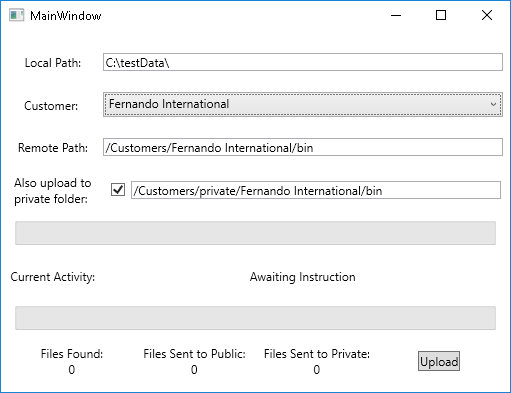
\includegraphics[width=0.75\textwidth]{FTPUploader}
		\caption{A Screenshot of the FTP Uploader application}
		\label{fig:FtpUploader}
	\end{figure}
	My first task was to create a FTP Uploader, this was to be used internally as a tool to upload releases of the application to an FTP server where it could then be accessed by the customers. The requirements for this tool were to:
	\begin{itemize}
		\item{Have a GUI for easy use}
		\item{Manage options for different releases}
		\item{Have an option to also upload the release to a private folder}
		\item{Automatically have values set based on defaults}
	\end{itemize} 
	The FTP Uploader was a good introduction into developing a MVVM application as it allowed me to get to grips with how the model works without too much complexity added from the application logic. I was then able to use this base knowledge about MVVM and WPF applications to develop GUI programs later on. This project still needs some work on it before it can be used. I have had to clean up the ticket for this project and add some more information on it so that it can be picked up by someone else after I leave.
}